\documentclass[10pt,a4paper]{article}
\usepackage[utf8]{inputenc}
\usepackage[french]{babel}
\usepackage[T1]{fontenc}
\usepackage{amsmath}
\usepackage{amsfonts}
\usepackage{amssymb}
\usepackage{makeidx}
\usepackage{graphicx}
\usepackage{subcaption}
\usepackage{lmodern}
\usepackage{verbatim}
\usepackage{hyperref}


\author{Aigret Julien \texttt{(8343-13-00)}\and Vanvyve Nicolas \texttt{(6590-13-00)}}
\date{16 mars 2016}
\title{LSINF1252\\Rapport de projet 1 :\\Implémentation de malloc, calloc et free}

\begin{document}

\maketitle

\section{Gestion de la mémoire}
\subsection{Initialisation}
Nous avons fait le choix d'initialiser notre \texttt{heap} à 1MB, taille qui semble raisonnable pour notre utilisation actuelle, mais qui eut être modifiée si besoin est. Cette limite n'est pas modifiée tout au long de l'éxécution de notre code.

\subsection{Fragmentation}
Dans notre programme, nous avons fait le choix d'allouer immédiatement une zone de mémoire (ou une combinaison de zones de mémoire) si elle est de la taille demandée par l'utilisateur. Dans le cas où il n'y a pas de zone de mémoire de taille précise, deux cas de figure se présentent : soit une ou des zones plus grandes ont été trouvées, ou aucune de taille suffisante n'a été trouvée. Dans le cas où une plus grande zone a été trouvée, nous gardons la plus grande de toutes et y installons notre zone de mémoire, créant un nouveau \texttt{block\_header} à la fin de celle-ci pointant sur la fin de la "zone libre".


\section{Tests unitaires}

Nous avons implémenté les tests unitaires décrits ci dessous via CUnit.
\begin{itemize}
	\item [$\bullet$] Myfree desalloc: nous vérifions que \texttt{alloc} de \texttt{block\_header} vaut bien 0.
	\item [$\bullet$] Mymalloc alloc : idem que ci dessus mais \texttt{alloc} de \texttt{block\_header} doit valoir 1
	\item [$\bullet$] Mycalloc alloc : idem que Mymalloc alloc
	\item [$\bullet$] Mymalloc size : nous vérifions que l'espace alloué correspond bien au multiple de 4 supérieur ou égal(en byte) de celui demandé.
	\item [$\bullet$] Mymalloc NULL : nous vérifions que si 0 byte sont demandé \texttt{mymalloc} renvoie \texttt{NULL}
	\item [$\bullet$] Mymalloc 2 alloc : nous vérifions que deux allocation successive via \texttt{mymalloc} ne pointe pas vers la meme adresse
	\item [$\bullet$] Mycalloc initialisation : nous vérifions que après un appel à \texttt{mycalloc} la mémoire allouée est bien initialisée à 0
\end{itemize}
Les test qui s'applique à \texttt{mymalloc} aurait pu etre transformés pour \texttt{mycalloc}. Mais étant donné que nous avons utilisé \texttt{mymalloc} pour implémenter le second cela ne servirait à rien.


\section{Tests comparatifs}

\begin{figure}
\centering

  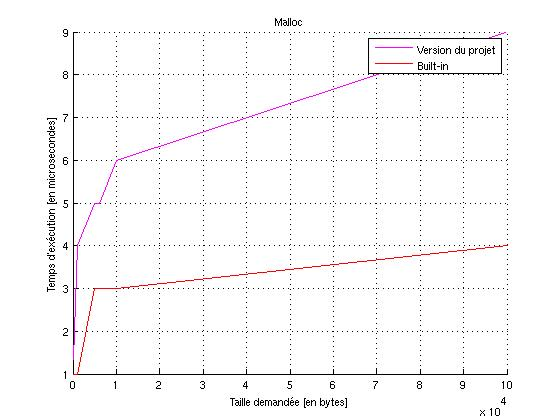
\includegraphics[width=1\linewidth]{graphe_malloc.jpg}
	\caption{Evolution de la vitesse d'allocation en fonction de la mémoire pour \texttt{malloc}}
  \label{fig1}
\end{figure}
\begin{figure}
  \centering
  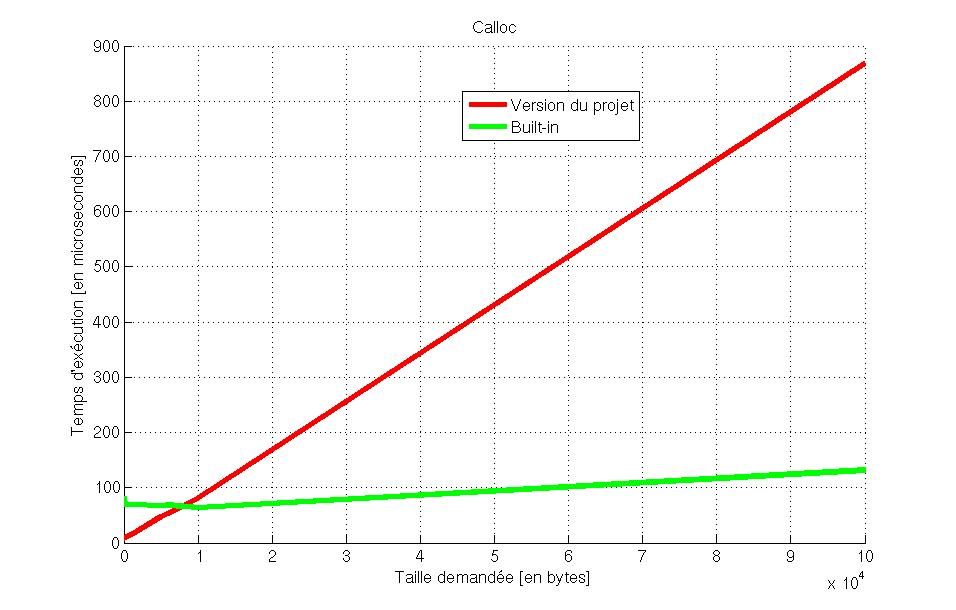
\includegraphics[width=1\linewidth]{graphe_calloc.jpg}
  \caption{Evolution de la vitesse d'allocation en fonction de la mémoire pour  \texttt{calloc}}
\label{fig2}
\end{figure}

Nous constatons, comme illustré sur les graphe (fig \ref{fig1} \& \ref{fig2}) que nos fonctions sont plus rapides pour les faibles allocations de mémoires, mais plus la mémoire devient grande et plus elles prennent du temps. Cela est certainement dû aux algorithmes de recherches utilisés par les fonctions \texttt{built-in} qui doivent être optimisés pour les grandes zones de mémoire. Notre initialisation de la zone mémoire par \texttt{calloc} est aussi très rudimentaire, et prend de plus en plus de temps au fur et à mesure que la taille de la zone à initialiser augmente.

\section{Difficultés rencontées}
Nous avons eu des difficultés avec la compréhension de la structure de \texttt{block\_header} comme décrite dans les consignes, ainsi que lors des précisions de consignes de la non-augmentaion du \texttt{heap}.
Le fonctionnement de \texttt{CUnit} a été compliqué à comprendre car mal expliqué dans les ressources du cours.

\section{Commentaires}
Les commentaires du codes sont intégralement dans le code.


\end{document}
